\documentclass[bibliography=totocnumbered]{scrartcl}
\usepackage{imakeidx}
\usepackage{ragged2e}
\usepackage{setspace} % Um den Zeilenabstand zu ändern.
\usepackage{gensymb}
%\usepackage{authblk}
% \usepackage{minitoc} % for the chpaters
\usepackage{wasysym}
%\usepackage{SI}
\usepackage{array} % Verwendung von Matrizen
\usepackage{booktabs} % Schöne Tabellen beziehungsweise sie sehen damit professioneller aus.
\usepackage{tabulary} % Ähnlich wie tabularx, ermöglicht aber das ändern der Ausrichtung der Spalten.
\usepackage{tabularx} % Tabellen mit automatischen Zeilenumbruch.
\usepackage{enumitem}
\usepackage{physics}
\usepackage[T1]{fontenc}% fontec und inputenc ermöglichen
\usepackage{graphicx}%Für Grafiken
\usepackage{rotating} % lässt Grafiken rotieren
\usepackage{mathtools}% mathematische Werkzeuge
\usepackage{amsmath}% Mathetools
\usepackage{amsfonts}% Mathetools
\usepackage{amssymb}% Symbole wie Natürliche Zahlen
\usepackage{geometry}
%\usepackage{bibtex} 
\usepackage{tablefootnote}% Fußnoten in Tabellen
\usepackage{float}% für eingebundene Bilder
\usepackage{fancyhdr} % Seiten schöner gestalten, insbesondere Kopf- und Fußzeile
\usepackage{ulem} 
\usepackage{dcolumn}% Align table columns on decimal point
\usepackage{bm}% bold math
\usepackage[ngerman]{babel} % Worttrennung nach der neuen Rechtschreibung und deutsche Bezeichnungen. babelfunktion wird wegen Literatur gebraucht.
\usepackage{subfloat} % Was macht diese Packet?
\usepackage{caption} % Unter-/Überschriften für Bilder, Grafiken und Tabellen
\usepackage{subcaption}
\usepackage{txfonts}
\usepackage{titling}% Titel
\usepackage[style=alphabetic]{biblatex} %biblatex mit alphabetic laden. alphbetic=Zitationsstil
\usepackage{bookmark}
\usepackage[printonlyused]{acronym}
\usepackage{amsthm}
\usepackage{pdfpages}
\usepackage{tikz}
\usepackage[siunitx,americanvoltages, europeanresistors,americancurrents]{circuitikz}
\usepackage{listings}
\usepackage{abstract}
\usepackage[per-mode = fraction]{siunitx}
\usepackage{hyperref}
\newcommand{\R}{\mathbb{R}} % reelle Zahlen
\newcommand{\N}{\mathbb{N}} % natürliche Zahlen
\newcommand{\C}{\mathbb{C}} % komplexe Zahlen
\newcommand{\Q}{\mathbb{Q}} % rationale Zahlen
\newcommand{\Z}{\mathbb{Z}} % ganze Zahlen
\newcommand{\F}{\mathbf{F}} % Kraft
\newcommand{\E}{\mathbf{E}} % Energie
\newcommand{\V}{\mathbf{v}} % Geschwindigkeit
\newcommand{\B}{\mathbf{B}} % magnetischer Fluss
\newcommand{\J}{\mathbf{j}} % Stromdichte ?
\newcommand{\D}{\mathbf{D}} % elektrische Induktion
\newcommand{\HH}{\mathbf{H}} % magnetische Feldstärke
\newcommand{\M}{\mathbf{M}} % Magnetisierung
\newcommand{\p}{\mathbf{P}}
\newcommand{\rr}{\mathbf{r}}
\newcommand{\vp}{\varphi}
\newcommand{\ve}{\varepsilon}
\newcommand{\vcc}[1]{\left(\begin{matrix}#1\end{matrix}  \right)}
\newcommand{\m}[1]{\left\lbrace #1\right\rbrace}
\newcommand{\los}{\noindent\textbf{Lösung}:}
\newcommand{\rang}[2]{\text{Rang}(#1)=#2}
\newcommand{\vpe}{\frac{1}{4\pi\ve_0}}
\newcommand{\qvpe}{\frac{q}{4\pi\ve_0}}
\newcommand{\geg}{\ac{geg.}}
\newcommand{\ges}{\ac{ges.}}

\newcommand{\kommando}[1]{$\backslash$\textit{#1}}
\newcommand{\com}[1]{$\backslash$\textit{#1}$\left\lbrace\ldots\right\rbrace$}
\newcommand{\Com}[2]{$\backslash$\textit{#1}$\left\lbrace #2\right\rbrace$}
\newcommand{\NeuKommando}[2]{$\backslash \textit{#1} \left\lbrace \backslash \textit{#2}\right\rbrace$}
\newcommand{\latex}{\LaTeX $\;$}


% si unitx
\DeclareSIUnit\litre{l}

\hypersetup{
	colorlinks=true,
	linkcolor=blue,
	filecolor=magenta,      
	urlcolor=cyan,
	citecolor=lime!50!black,
	filecolor=red
}
%\addbibresource{} %Bibliographiedateien laden
\addbibresource{bib.bib}

\geometry{a4paper, left=25mm, right=25mm, top=30mm, bottom=30mm}
\lhead{\thedate}
\rhead{GPR}
\lhead{\thetitle}
\pagestyle{fancy}

\usetikzlibrary{patterns}
\usetikzlibrary{3d}
\makeindex[title=Stichwortverzeichnis,intoc
,options= -s Index-Formatierung.ist
]
\author{Ben J. F.}
\allowdisplaybreaks

\lstset
{ %Formatting for code in appendix
    basicstyle=\footnotesize,
    numbers=left,
    stepnumber=1,
    showstringspaces=false,
    tabsize=2,
    breaklines=true,
    breakatwhitespace=false,
}



\title{T1 \\ Wärmekapazität eines Kalorimeters}
\date{16.06.2021}

\pagestyle{fancy}
\rfoot{T1}

\begin{document}
	\newgeometry{left=14mm, right=13.5mm, top=60mm, bottom=30mm}
	\begin{titlepage}
		\begin{center}
			{\huge{Grundpraktikum}}\\\vspace*{15mm}
			{\huge{\textbf{\thetitle}}}\\\vspace*{20mm}
			{\theauthor}\\\vspace*{10mm}
			{\thedate}\\\vspace*{40mm}
			
			
			
		\end{center}
	\end{titlepage}
	\makeatother
	\restoregeometry
	\newpage
	
	\tableofcontents
	\newpage
	
	\listoffigures 
	\listoftables
	\newpage
	
	
	
	\section{Motivation und theoretische Vorbetrachtung}
	% Versuchziel: Was will ich mit dem Versuch erreichen?
	% Aufgabenstellung
	% theoretische Einführung: Wie sieht die Physik dahinter aus (Knapp fassen)? Welche Formeln verwende ich? Wie ist der Versuch aufgebaut (Skizze, Abbildungen etc)? Welche Einheiten kommen vor?
	
	Ziel des Experimentes ist es die spezifische Wärmekapazität des Behälters, oder auch Kalorimeter
	genannt, auszurechnen, da die Wärme nicht nur von dem Medium, hier Wasser, aufgenommen
	wird, sondern ebenso von dem Kalorimeter aufgenommen wird.
	\\
	\\
	Um dies zu tun werden zwei verschiedene Verfahren verwendet.
	Die elektrische Methode, wo durch eine Heizspirale die den Widertand R besitzt und über die die
	Spannung U und Stromstärke I angeschlossen, Wasser mit der Temperatur T und Volumen V erhitzt.
	Im einem Zeitintervall misst man dann die Temperatursteigerung und bestimmt mit Hilfe der
	Gleichung den Kalorimeterwert.
	\begin{equation}\label{eq: elektrische Methode}
	C_{k}	=\dfrac{U\cdot I \cdot \Delta}{\Delta T } t-m_{w}\cdot c_{w}
	\end{equation}
	Die zweite Methode ist die Mischmethode, wo Wasser mit dem Volumen V1, sowie einer niedrigen
	Temperatur T1 und Wasser mit dem Volumen V2 einer höheren Temperatur T2. Durch das
	thermische Gleichgewicht entsteht eine Mischtemperatur, die jedoch geringer ist, da Wärme ebenso
	durch den Kalorimeter aufgenommen wurde.
	Daraus ergibt sich der Zusammenhang:
	\begin{equation}\label{eq: Mischungsmethode}
		C_{k}=m_{2}\cdot c_{w}\dfrac{(T_{2}-T_{w})}{(T_{m}-T_{1}) }-m_{1}\cdot c_{w}
	\end{equation}
	
	
	\section{Elektrische Methode}
	
	\subsection{Durchführung}
	Es wurde eine Wärmeaustauschkorrektur durchgeführt. Dafür wurde vor und nach dem
	Heizen 5 Minuten jede Minute die Temperatur gemessen, diese werden hier als Vor- und
	Nachperiode bezeichnet.\\
	In der Hauptperiode werden für 5 Minute das Wasser geheizt und durch einen Motor die Wärme
	verteilt wird. Dabei wird alle 10 Sekunden die Zeit gemessen.
	Dabei wird die konstante Spannung und Stromstärke wie in der Tabelle angelegt.\\
	
	\begin{table}[ht!]
		\centering
		\caption[Spannung,Strom]{gemessene Werte für Stromstärke und Spannung}
		\begin{tabular}{|c||c|c|}
			\hline
			\textbf{Messung} & \textbf{Experimentatorin} & \textbf{Experimentator} \\
			\hline
			\hline
			\multicolumn{3}{|c|}{\textit{Spannung}[V]} \\
			\hline
			\hline
			1 & $ 25.5\pm0.1 $ & $ 24.8\pm0.3 $ \\
			\hline
			2 & $ 25.5\pm 0.1 $ & $ 25.0 \pm0.3 $\\
			\hline\hline
			\multicolumn{3}{|c|}{\textit{Stromstärke}[A]} \\
			\hline\hline
			1 & $ 4.00\pm0.05 $ &$ 3.00\pm0.05 $  \\
			\hline
			2 & $ 4.00\pm0.05 $ & $ 3.00\pm0.05 $ \\
			\hline
		\end{tabular}
		\label{tab: Spannung, Strom}
	\end{table}
	\newpage
	\subsection{Datenauswertung}
	In dem Anhang sieht man die gemessen Werte von T, U, I in Abhängigkeit von t angegeben.
	Nun wurde die lineare Regression für die Vor, Nach und Hauptperiode mit den Gleichungen, gemäß
	dem Versuchsskript\smartcite{Muller.c} .
	\begin{align}
		f_{vor}=at+b\\
		f_{haupt}=ct+d\\
		f_{nach}=et+f
	\end{align}
	
	Die Daten der liniearen Regression wurden in folgenden Graphen zusammen gefasst.
	
	\begin{figure}[ht!]
		\centering
		\begin{minipage}[ht!]{0.45\linewidth}
			\centering
			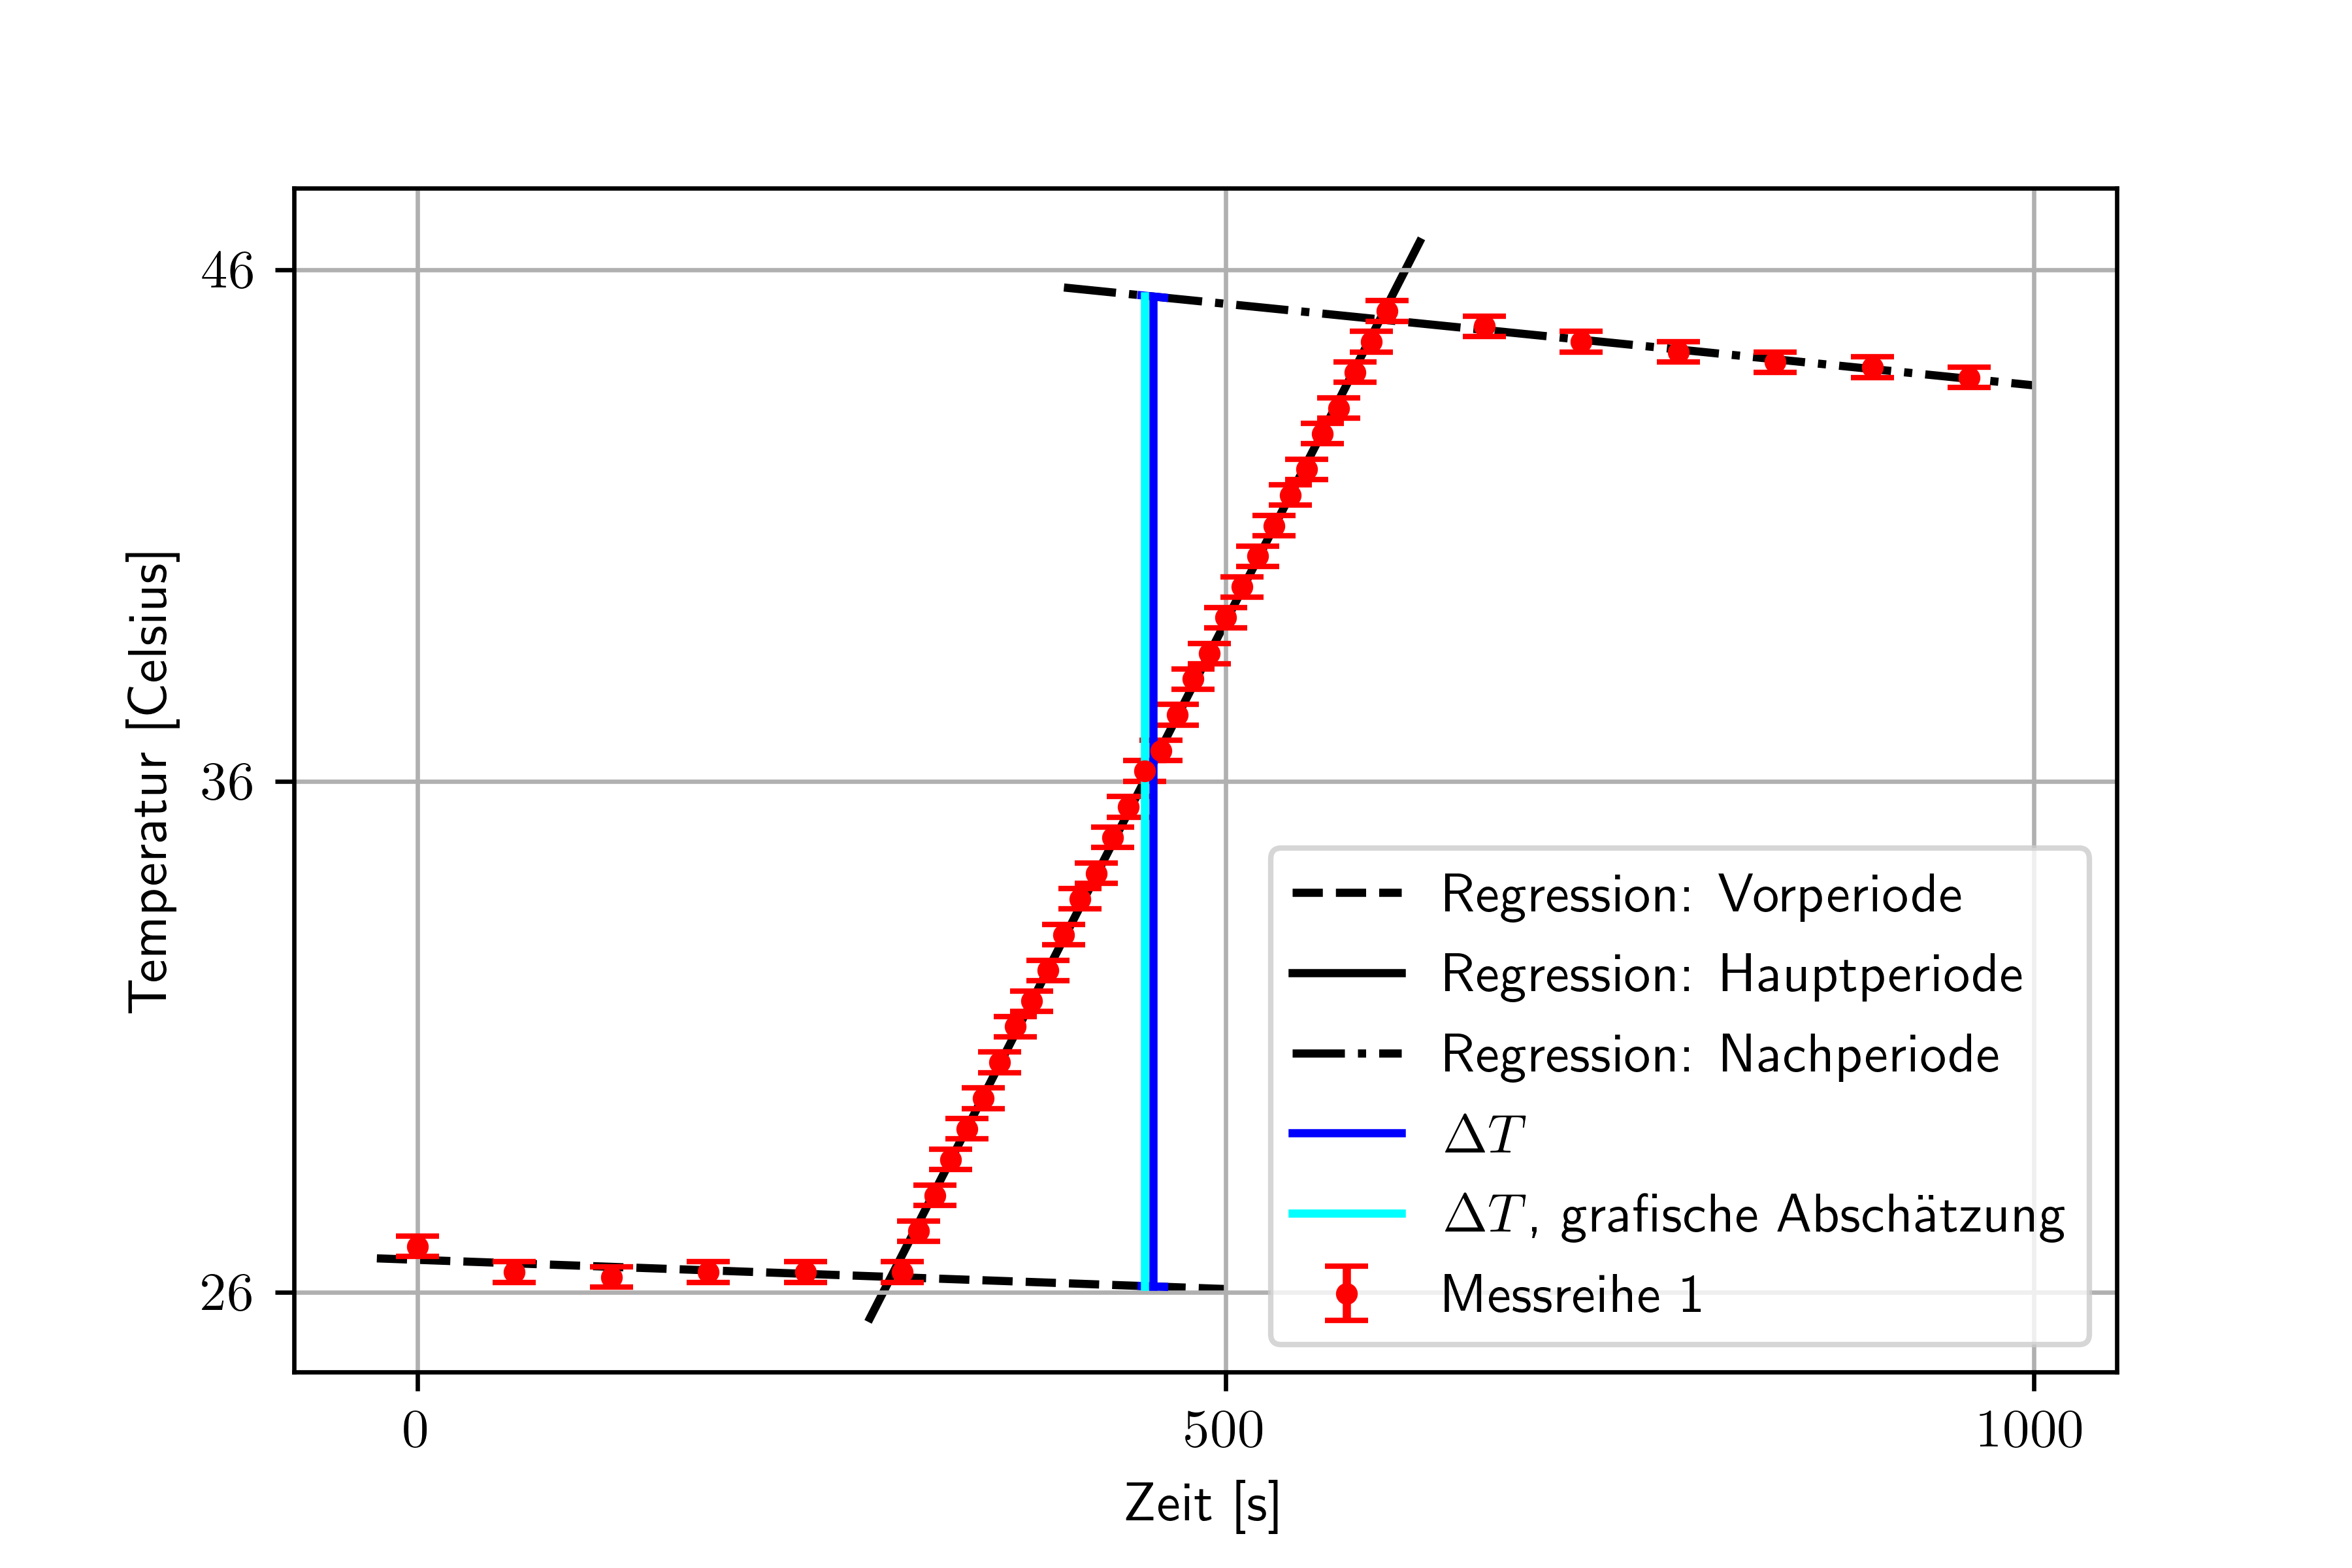
\includegraphics[width=\textwidth]{fotos/gpr1/M1_T1.png}
			\caption[Messreihe 1.1]{Messreihe 1; Vor-, Haupt- und Nachperiode; Ben }
			\label{Abb: M1 Ben}
		\end{minipage}
		\hfill
		\begin{minipage}[ht!]{0.45\linewidth}
			\centering
			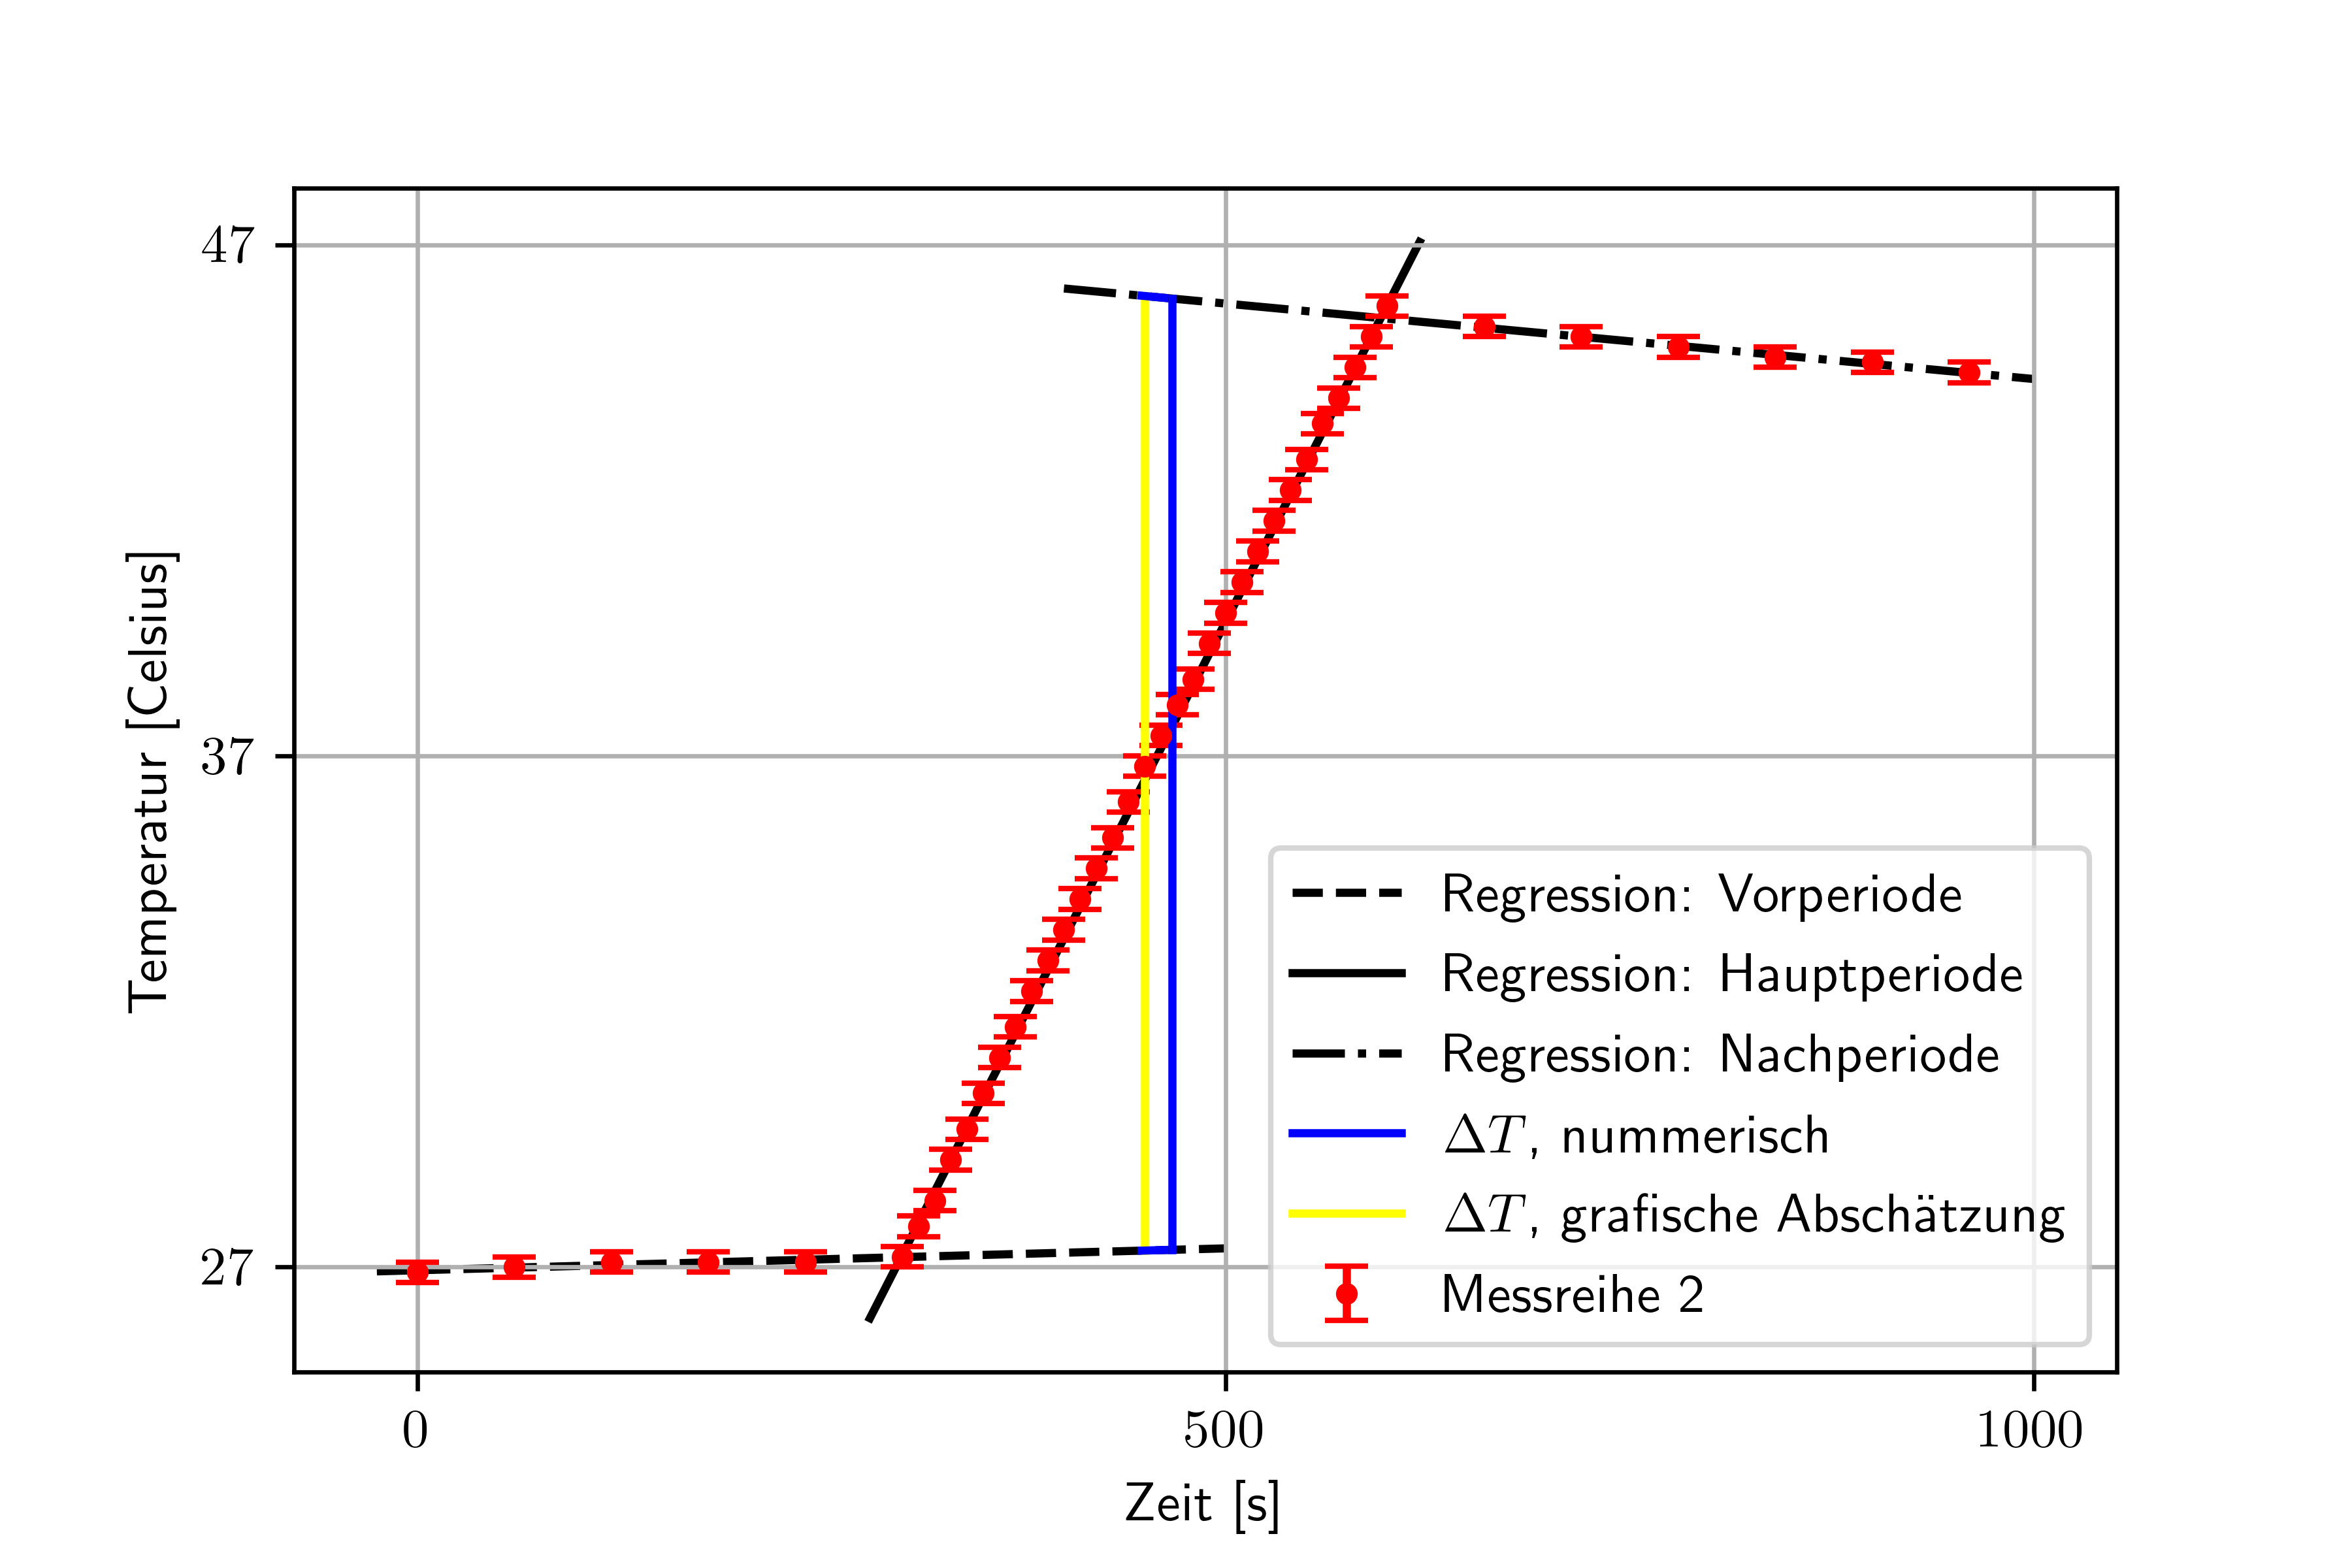
\includegraphics[width=260pt]{fotos/gpr1/M2_T1.png}
			\caption[Messreihe 2.1]{Messreihe 2; Vor-, Haupt- und Nachperiode; Ben}
			\label{Abb: M2 Ben}
		\end{minipage}
	\end{figure}

	\begin{figure}[ht!]
		\centering
		\begin{minipage}[ht!]{0.45\linewidth}
			\centering
			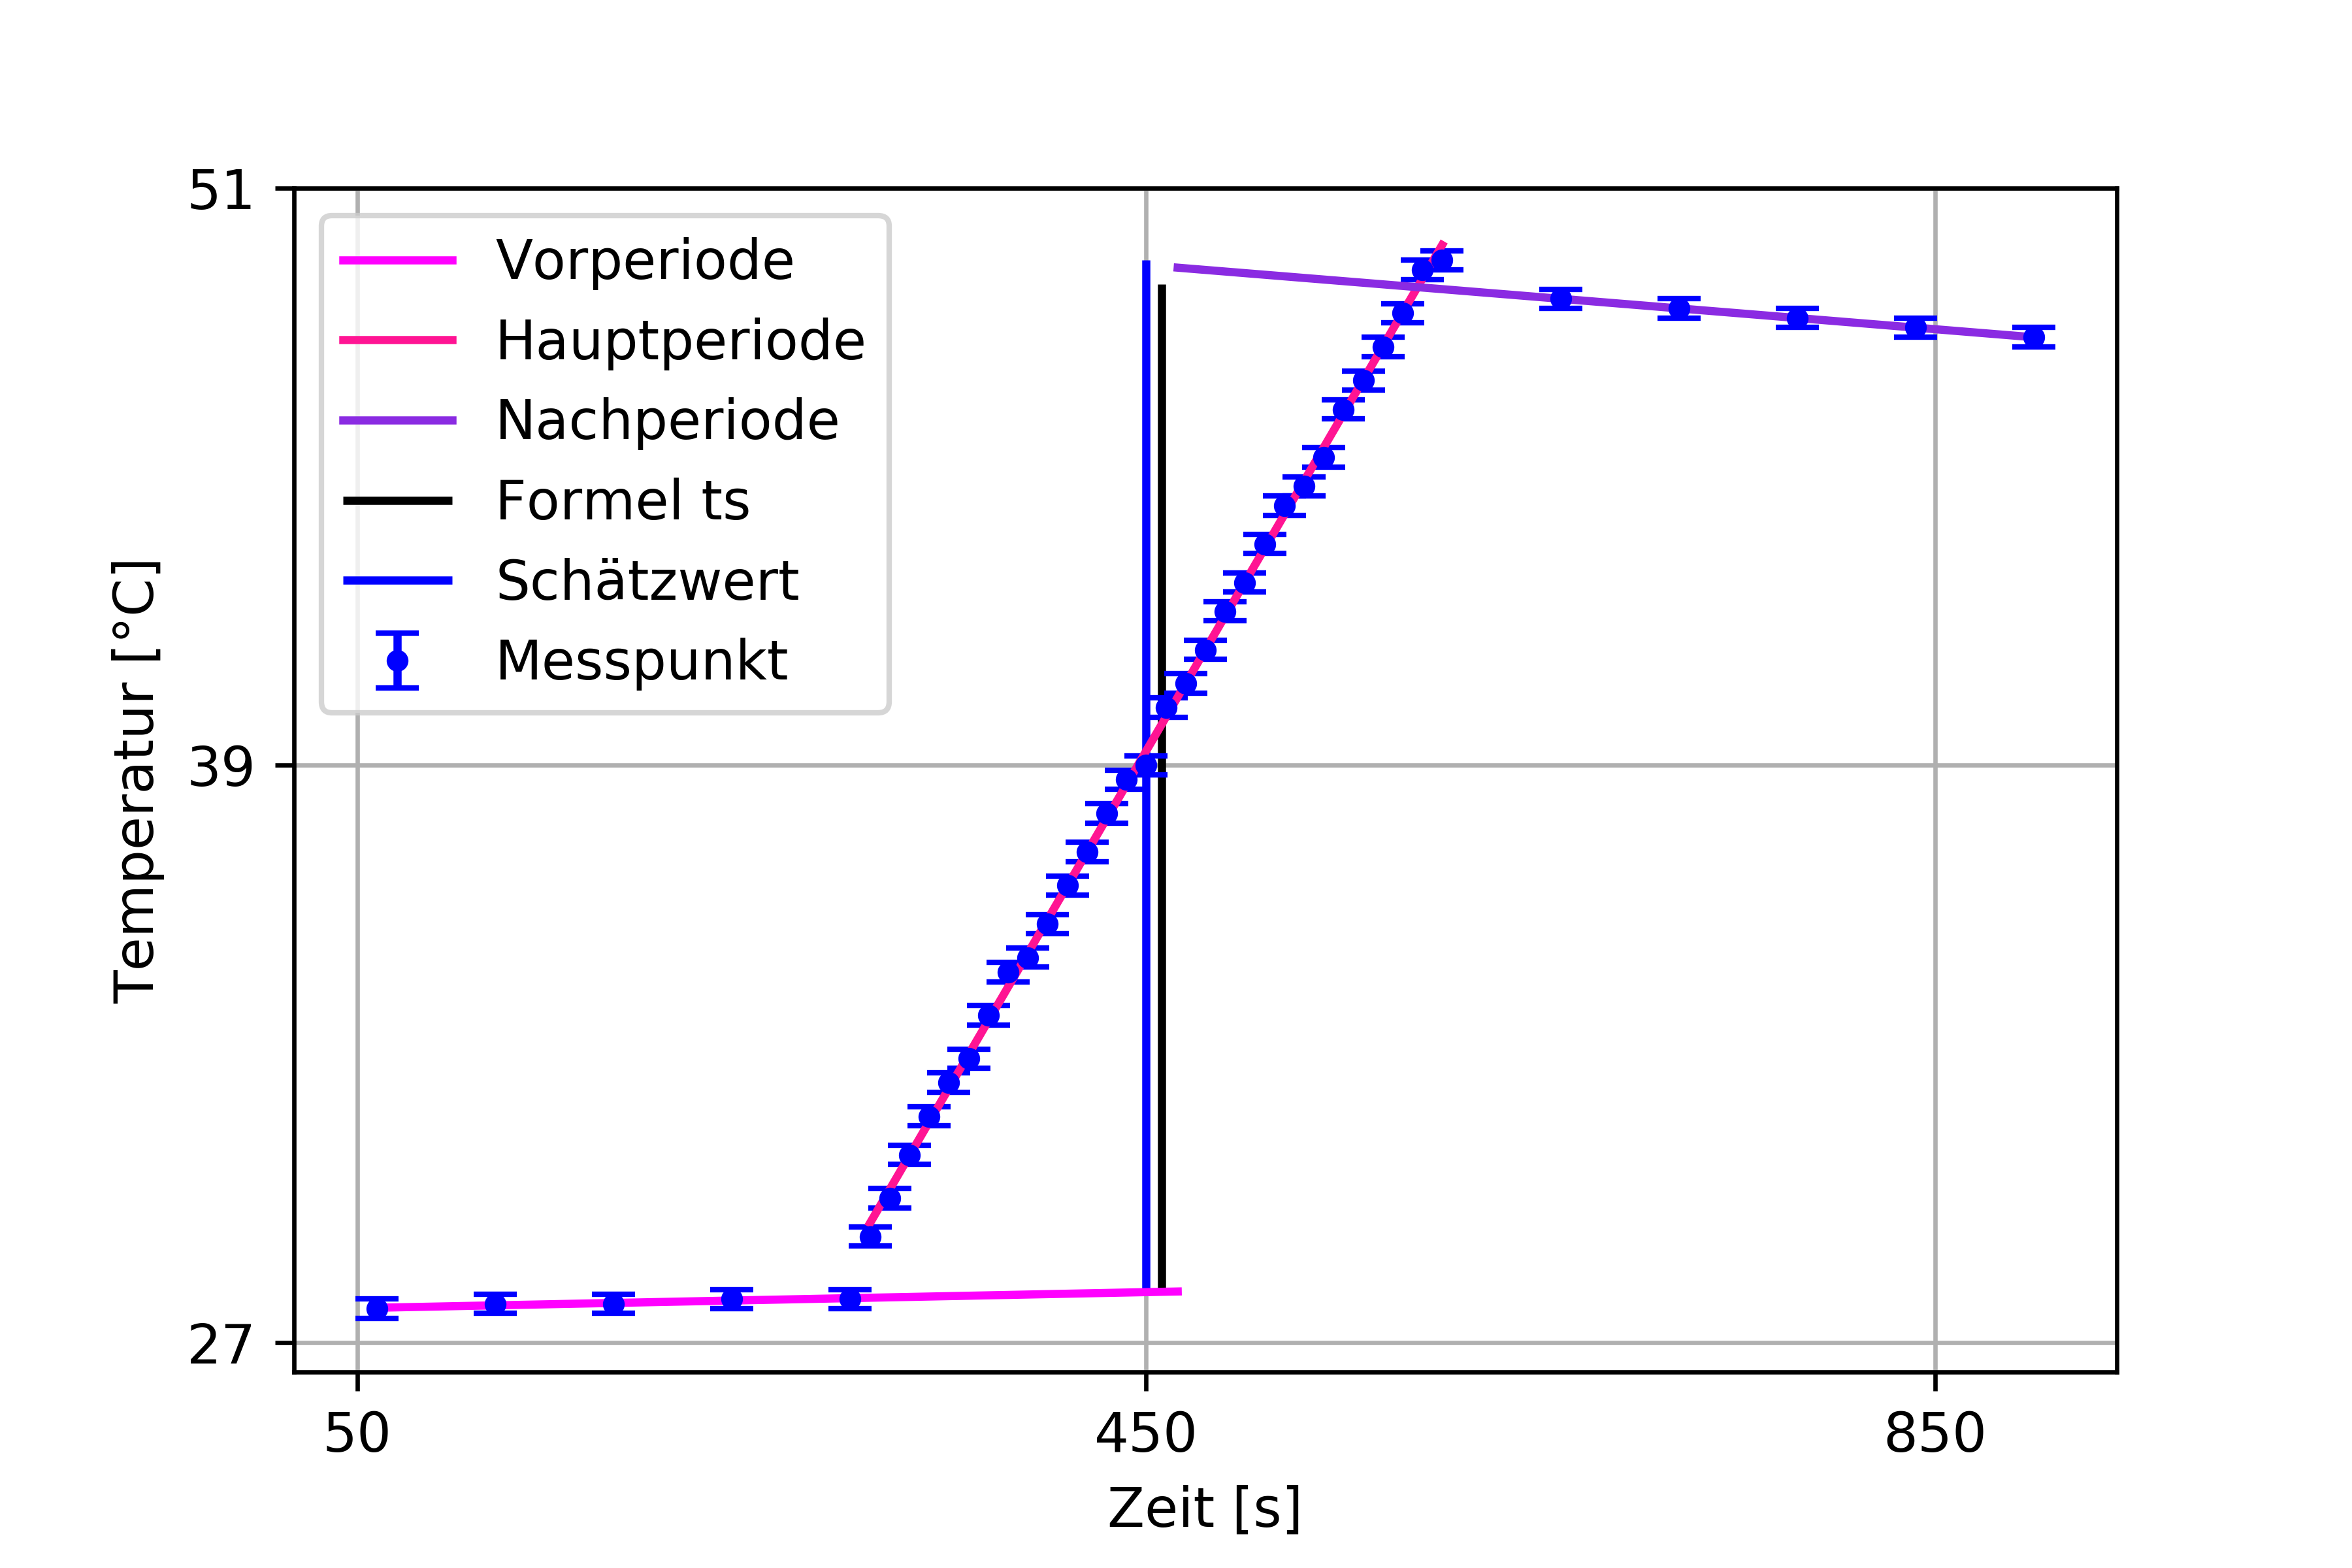
\includegraphics[width=260pt]{fotos/gpr1/S_T1_M1.png}
			\caption[Messreihe 1.2]{Messreihe 1; Vor-, Haupt- und Nachperiode}
			\label{Abb: M1 Sara}
		\end{minipage}
		\hfill
		\begin{minipage}[ht!]{0.45\linewidth}
			\centering
			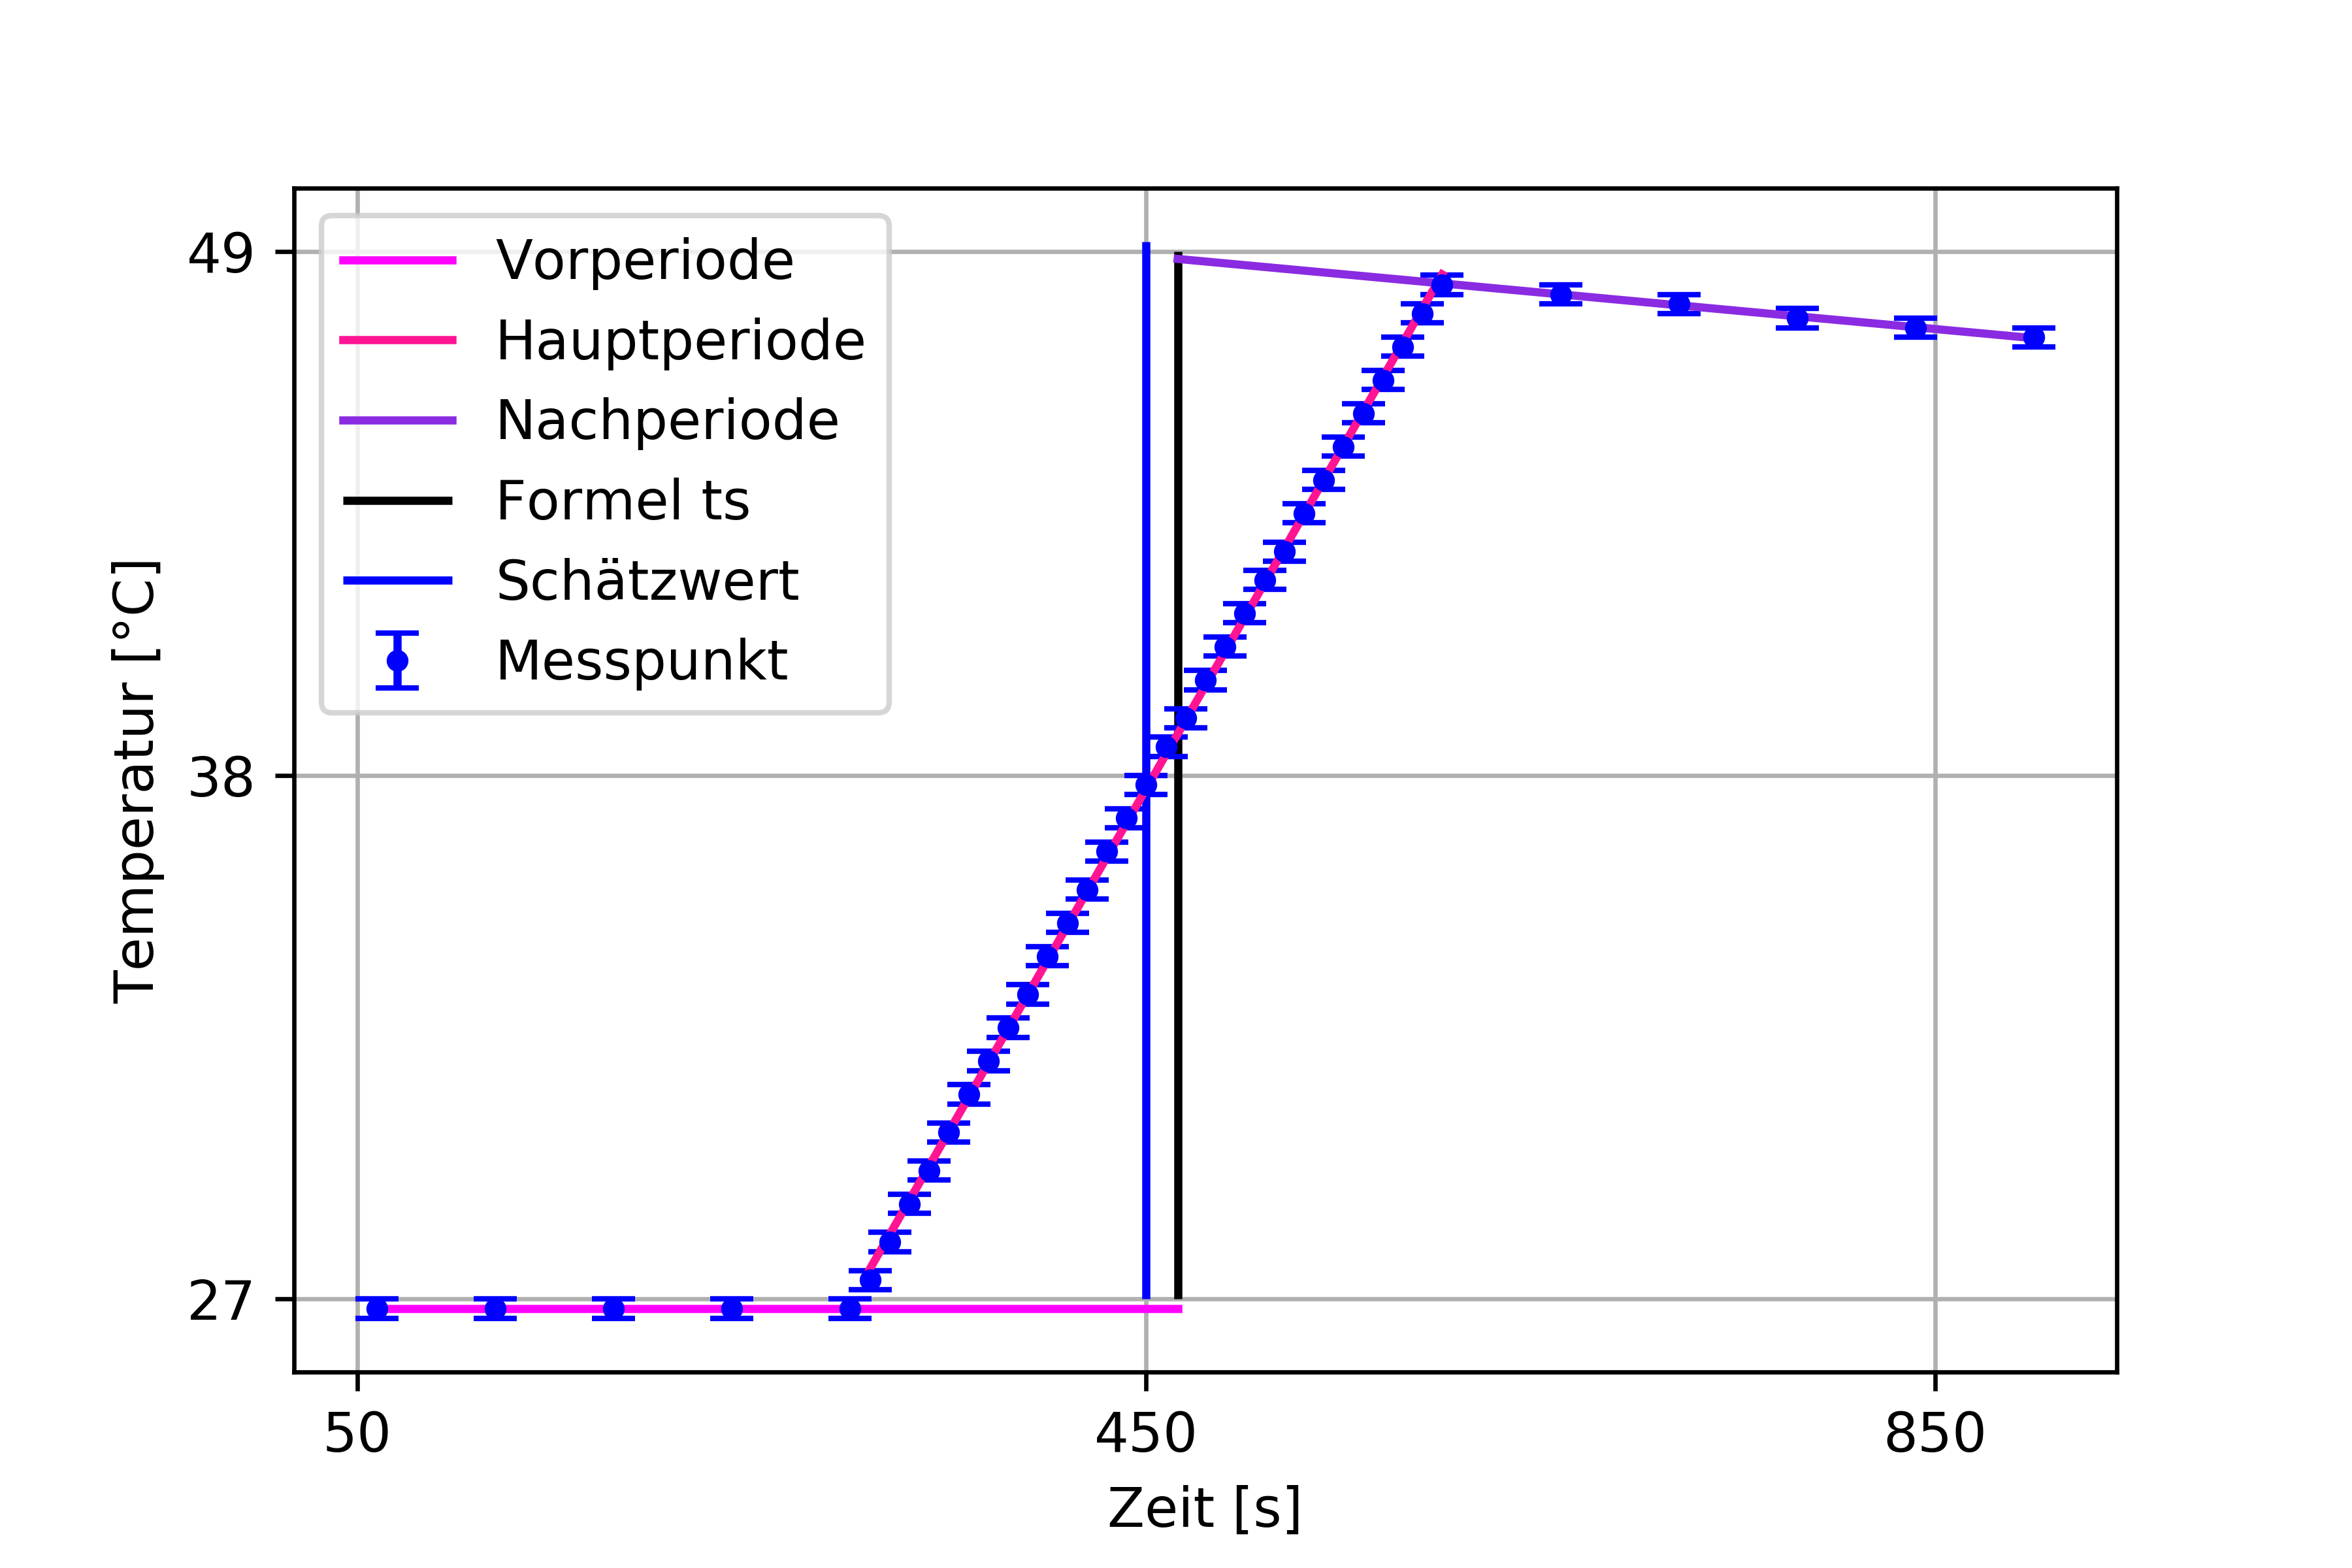
\includegraphics[width=260pt]{fotos/gpr1/S_T1_M2.png}
			\caption[Messreihe 2.2]{Messreihe 2; Vor-, Haupt- und Nachperiode}
			\label{Abb: M2 Sara}
		\end{minipage}
	\end{figure}
	\newpage


	Die liniearen Zusammenhänge konnten somit bestätig werden.
	Dabei kamen die Parameter der linearen Regressionen werden in folgender Tabelle eingefügt.
	\begin{table}[ht!]
		\centering
		\caption[Regressionsparameter]{Regressionsparameter, gemittelt}
		\begin{tabular}{|c||c|c|}
			\hline
			\textbf{Parameter} & \textbf{Korrektur I} & \textbf{Korrektur II }\\
			\hline\hline
			\multicolumn{3}{|c|}{\textit{Vorperiode}} \\
			\hline\hline
			$ a $ [$ ^{\circ} $Cs$ ^{-1} $] & $ (4.2\pm 0.8)\cdot 10^{-4}$  &$(1 \pm 4)\cdot 10^{-4}$  \\
			\hline
			$ b $ [$ ^{\circ} $C] & $ 27.23\pm0.32 $ &$ 26.79\pm 0.07$  \\
			\hline\hline
			\multicolumn{3}{|c|}{\textit{Hauptperiode}} \\
			\hline\hline
			$ c $ [$ ^{\circ} $Cs$ ^{-1} $]& $(7.106\pm0.020)\cdot 10^{-2}  $ & $(62.04\pm 0.15)\cdot 10^{-2} $ \\
			\hline
			$ d $  [$ ^{\circ} $C]& $6.53 \pm 0.09$ &$ 8.41\pm0.07 $  \\
			\hline\hline
			\multicolumn{3}{|c|}{\textit{Nachperiode}} \\
			\hline\hline
			$ e $ [$ ^{\circ} $Cs$ ^{-1} $] & $-(3.58 \pm0.08 )\cdot 10^{-3}$ & $ -(3.07\pm 0.013)\cdot 10^{-3}$ \\
			\hline
			$ f $  [$ ^{\circ} $C]& $50.77 \pm0.07 $ & $ 47.13\pm 0.11$ \\
			\hline
		\end{tabular}
		\label{tab: Parameter}
	\end{table}
	
	
	\subsection{Berechnung der Temperaturdifferent und \\ der Wärmekapazität des Kalorimeters}
	
	Aus dem Versuchsskript\smartcite{Muller.c} wurden die Zeiten der Schnittpunkte der Vor und Nachperiode mit der Hauptperiode. 
	\begin{align}
		t_{B}=\dfrac{d-b}{a-c}\\
		t_{E}=\dfrac{f-d}{c-a}
	\end{align}
	Und als Zeit\smartcite{Muller.c}, wo die Flächen zwischen der waagerechten und dementsprechenden Dreiecken der
	Hauptperiode, mit der Vor oder Nachperiode.
	\begin{equation}\label{eq: ts}
		t_{s}=\dfrac{\dfrac{d-b}{a-c}\cdot \sqrt{c-a}+\dfrac{f-d}{c-a} \cdot \sqrt{c-e}}{\sqrt{c-a}+\sqrt{c-e}}
	\end{equation}
	Damit ergibt sich als Temperaturdifferenz:
	\begin{equation}\label{eq: Temperaturdifferenz}
		\Delta T= (e-a)t_{s}+(f-b)
	\end{equation}
	\newpage
	Die Wärmekapazität des Kalorimeter ergibt sich durch (\ref{eq: elektrische Methode}) mit der Zeitdifferenz als Wert der Dauer
	der Hauptperiode.
	Somit ergeben sich die Werte und ihre Unsicherheiten gemäß der Gauß'scher Fehlerfortpflanzung.
	\begin{table}[ht!]
		\centering
		\caption[Wärmekapazität]{Wärmekapazität des Kalorimeters nach elektrischer Methode mit gemittelten Parametern}
		\begin{tabular}{|c||c|c|}
			\hline
			\textbf{Formelzeichen} & \textbf{Experimentatorin} & \textbf{Experimantator} \\
			\hline\hline
			$ t_{B} $ [s]& $  293 $ & $  295.6 $ \\
			\hline
			$ t_{E} $ [s]& $  626 $ & $ 623  $ \\
			\hline
			$ t_{s} $ [s]& $  461 $ & $  461 $ \\
			\hline
			$ \Delta T $ [$ ^{\circ} $C]& $ 22.0\pm 0.5$ &$ 19.3\pm 0.4$  \\
			\hline
			$ C_{k} $&$ 155\pm28 $  & $ 140\pm 40 $ \\
			\hline
		\end{tabular}
		\label{tab: Ck nach el. Meth.}
	\end{table}
	
	\subsection{Auflistung der Unsicherheiten}
	Dabei besitzen die Gerätewerte die folgenden zufällige, durch Geräteunsicherheit und
	Größtfehlerabschätzung der Ableseungenauigkeit, und systematischen Fehler, durch
	Genauigkeitsangaben der Messgeräte.
	
	\begin{table}[ht!]
		%\centering
		\hspace{-1cm}
		\caption[Messunsicherheiten 1]{Messunsicherheiten der elektrischen Methode.\\ Die Nummerierung 1 und 2 stehen für Experimentatorin und Experimentator. Rz=Reaktionszeit. Vm=Voltmeter. Am=Amperemeter. Stu=Stoppuhr. \\DTm= Digital Thermomenter. Die Gleichungen für die Unsicherheiten wurden im Skript\protect\cite{Muller.} nachgeschlagen.}
		\begin{tabular}{|c||c|c|c|c|}
			\hline
			\textbf{Unsicherheit} & \textbf{Temperatur} [$ ^{\circ} $C] & \textbf{Zeit} [s] & \textbf{Spannung} [V]& \textbf{Strom} [A]\\
			\hline\hline
			\textit{systematische} &$ u_{last-Digit} =\pm 0.01  $  & $  u_{Stu}=5\cdot 10^{-4} T $ &$  u_{Vm,1}=\pm0.1 $  & $ u_{Am,1,2}=\pm 0.05  $   \\
			\textit{Unsicherheiten} & $ u_{DTm}=\pm T\cdot 10^{-3}  $ & $ u_{last-Digit}=\pm 0.01  $ &$  u_{Vm,2}=\pm0.3 $  & --\\
			\hline\hline
			\textit{statistische} & $   $ & $  u_{Rz,1,2}=\pm0.3  $ & -- &  -- \\
			\textit{Unsicherheiten}  &$   $  & $  $ &--  & --  \\
			\hline
		\end{tabular}
		\label{tab: M.u.1}
	\end{table}
	
	
	\section{Mischmethode}
	\subsection{Durchführung}
	In dem Kalorimeter wurde eine Wassermenge von 150ml mit ca. Zimmertemperatur eingefügt und
	anschließend eine erhitzte Wassermenge des selben Volumens.
	Anschließend wird der Motor angeschalten , damit es schneller zum thermischen Gleichgewicht kam.
	Mittels der Richmannschen Mischungsregel wird dann die Wärmekapazität des Kalorimeters.
	\newpage
	\subsection{Datenauswertung}
	Dabei wurden die folgenden Werte aufgenommen.
	
	\begin{table}[ht!]
		\centering
		\caption[Daten]{gemittelte Daten der Mischungsmethode}
		\begin{tabular}{|c||c|c|}
			\hline
			\textbf{Formelzeichen} & \textbf{Experimantorin} & \textbf{Experimentator} \\
			\hline\hline
			$ T_{1} $ [K] & $300.18 \pm0.12 $ & $ 299.82\pm0.12 $ \\
			\hline
			$ T_{2} $ [K]& $316.68 \pm 0.12$ &  $ 313.22\pm 0.12$\\
			\hline
			$ T_{M} $ [K]& $ 307.22\pm 0.12$ & $ 305.75\pm0.12 $ \\
			\hline
			$ V_{1} $ [kg] &$ 0.1500\pm 0.0012$  &$ 0.1487\pm0.0012 $  \\
			\hline
			$ V_{2} $ [kg]& $ 0.1500\pm 0.0012$ &$0.1483 \pm0.0012 $  \\
			\hline
		\end{tabular}
		\label{tab: Daten Mischungsmethoden}
	\end{table}
	
	\subsection{Berechnung der Wärmekapazität}
	Mit der Gleichung (\ref{eq: Mischungsmethode}) kommt als Wärmekapazität des Kalorimeters folgende Werte:
	
	\begin{table}[ht!]
		\centering
		\caption[Wärmekapazität]{Messergebnisse für die Wärmekapazität nach der Mischungsmethode}
		\begin{tabular}{|c||c|c|}
			\hline
			\textbf{Messreihe} & \textbf{Experimentatorin} & \textbf{Experimenator} \\
			\hline\hline
			1 & $ 220\pm30 $ &$ 110\pm60 $  \\
			\hline
			2 & $ 210\pm90 $ & $ 190\pm 50$ \\
			\hline
			3 & $ 230\pm60 $ & $170 \pm 70$ \\
			\hline
		\end{tabular}
		\label{Abb: Wärmekapazität Mischungsmethode}
	\end{table}
	
	
	\section{Vergleich}
	
	Aus der Mischmethode und der elektrischen Methode konnten folgende Werte ermittelt werden.\\\\
	\begin{table}[ht!]
		\centering
		\caption[Vergleich]{Vergleich der Wärmekapazitäten des Kalorimeters}
		\begin{tabular}{|c||c|c|}
			\hline
			\textbf{Messreihe} & \textbf{Experimentatorin} & \textbf{Experimentator} \\
			\hline\hline
			\multicolumn{3}{|c|}{\textit{elektrische Methode}} \\
			\hline\hline
			1 & $ 180\pm40 $ & $120 \pm 40$ \\
			\hline
			2 & $ 130\pm 40$ &$ 150\pm40 $  \\
			\hline\hline
			\multicolumn{3}{|c|}{\textit{Mischungsmethode}} \\
			\hline\hline
			1 & $ 220\pm30 $ &$ 110\pm60 $  \\
			\hline
			2 & $ 210\pm90 $ & $ 190\pm 50$ \\
			\hline
			3 & $ 230\pm60 $ & $170 \pm 70$ \\
			\hline\hline
			\multicolumn{3}{|c|}{\textit{Mittelwerte}} \\
			\hline\hline
			& $192 \pm 25$ & $ 148\pm 24$ \\
			\hline
		\end{tabular}
		\label{tab: Vergleich}
	\end{table}
	\\\\
	Alle Werte scheinen mit ihren Unsicherheiten sich zu überschneiden und somit in demselben Wertebereich zu
	liegen, auch wenn die Werte der Mischmethode deutlich höher liegt. Die Unsicherheiten scheinen bei beiden jedoch sehr groß zu sein.
	
	\section{Fehlereinschätzung}
	
	 \subsection{Waagerechtes Ablesen}
		Durch die Digitalem Anzeigen und der Spiegelskala wurde der Ablesefehler möglichst klein gehalten und hat kaum Auswirkungen auf die Unsicherheiten und dem Wert.
		 \subsection{Volumenmessung}
		Das Messen des Volumes ist aufgrund der Oberflächenspannung fehlerhaft. Außerdem bleibt noch
		etwas im dem Messzylindern. Doch wurde 3ml als Fehler genommen, was ausreichend ist, auch
		wenn es die Unsicherheit größer werden lässt.
		 \subsection{Dichte Wasser}
		Es wurde angenommen, dass man die Masse und Volumen auf Grund der Dichte gleich fehlerlos
		setzten könnte. Die Dichte ist jedoch Temperatur abhängig. Jedoch ist es nahezu identisch, da die
		Dichte nahezu $ 1000 $ kg m$ ^{-2} $ beträgt und die Differenzen von $ 20 $ K kaum von belangen ist. Jedoch ist
		es keine fehlerlose Annahme. 
		\subsection{ Wechselwirkung mit der Umgebung, isoliertes System}
		Bei der elektrischen Messmethode wurde die Wärmeaustauschkorrektur gemacht, weshalb dort
		genau der Umstand der Wechselwirkung mit der Umgebung von dem Wert korrigiert wird.\\\\ Bei der Mischmethode hingegen wurde diese Wechselwirkung gemessen, jedoch wurde die gesamte
		Wärmemenge die aus dem System gelangt gemessen, was auch einen Teil beträgt der nicht in dem
		Kalorimeter fließt sondern in die Umgebung, zum Bespiel dem Rührer, Motor, Thermometer. Somit
		kann man nicht von einer isolierten System ausgehen, was die Werte zu groß werden lässt bei der
		Mischmethode.\\\\Außerdem könnte auch ein Effekt haben, dass der Kalorimeter noch nicht ganz abgekühlt war, als
		man das Experiment wiederholt hatte, bzw. zur Mischmethode nach der elektrischen Methode kam.
		Somit würde weniger Wärme aufgenommen werden und die Wärmekapazität des Kalorimeter
		kleiner.

	
	
	\section{Schlussfolgerung}
	Aufgrund der Wärmeaustauschkorrektur schein die elektrische Methode die genauere zu sein,
	trotzdem die Unsicherheit hoch liegt, aufgrund der vielen fehlerbehafteten Größen für die
	Berechnung. Man könnte den Fehler dezimieren indem man den Computer die Messungen
	durchführen lässt, denn so würden beispielsweise die Reaktionszeit und die (wenn auch geringen)
	Ablesefehler wegfallen.\\\\
	Bei der Mischtemperatur wäre es von Vorteil den Kalorimeter besser von der Umgebung zu isolieren,
	denn zum Beispiel für das Loch für den Thermometer gibt es direkten Kontakt mit der Umgebung.
	Um präzisere Werte zu bekommen könnte man alle Gerätschaften (Motor, Kalorimeter, Thermometer
	etc.) ebenso auf eine festgelegte gleiche Temperatur gebracht werden, bevor ein neues Experiment
	gestartet wird, um gleiche Ausgangsbedingungen zu haben.\\\\
	Allgemein wäre es ebenso genauer statt des Volumens die Masse zu messen, da eine digitale Wage
	einen geringeren Fehler besitzt und somit auch Ablesefehler durch Oberflächenspannung entgegen
	gewirkt werden.\\\\
	Alles im Allem scheint die Hypothese des Experimentes mit den Zusammenhängen der Gleichungen
	zur Wärmekapazität des Kalorimeters bestätigt und das Experiment kann als gelungen angesehen
	werden. 
	
	
	
	

	\section{Fragen aus dem Skript: T1 }
	Die Wärmekapazität $ C_{k} $ des Kalorimeters ist von der eingefüllten Wassermenge und der Temperatur aufgrund der Energieerhaltung abhängig.\footnote{Erste Frage \smartcite[vgl.][77]{Muller.c}: Weshalb ist die Wärmekapazität $ C_{k} $ des Kalorimeters von der eingefüllten Wassermenge und der Temperatur abhängig?} Die Menge des Wasser beeinflusst die maximale Energie, welche gespeichert werden kann und die Temperatur gibt an, wie viel Energie gespeichert ist. Diesen Zusammenhang können wir in beiden Gleichungen(\ref{eq: elektrische Methode}, \ref{eq: Mischungsmethode}) beobachten. Denn beide stellen die Energieerhalung dar.\\\\
	\footnote{Zweite Frage \smartcite[vgl.][77]{Muller.c}: Warum ist für die Mischungsmethode keine Wärmeaustauschkorrektur erforderlich?}Die Mischungsmethode basiert darauf, dass sich zwei gleich große Mengen von Wasser mit unterschiedlichen Temperaturen vermischen. Hierbei findet eine gewollter Wärmeaustausch statt. Bei der Wärmeaustauschkorrektur wollen wir unser Ergebnis von dem ungewollten Wärmeaustausch mit der Umgebung bereinigen. Daraus lässt sich schließen, dass die Wärmeaustauschkorrektur nicht erforderlich ist.\\\\
	"Der Wert der spezifischen Wärmekapazität für Wasser isr relativ groß im Vergleich zu anderen Flüssigkeiten und Festkörpern."\smartcite[vgl.][77]{Muller.c}\footnote{Dritte Frage  \smartcite[vgl.][77]{Muller.c}: Der Wert der spezifischen Wärmekapazität für Wasser isr relativ groß im Vergleich zu anderen Flüssigkeiten und Festkörpern. Welche Bedeutung ha dies für das Klima?} Dadurch können die Ozeane viel Energie speichern, ohne sich schnell zu erwärmen. Aufgrunddessen ändert sich das Wassersystem im Meer sehr langsam und klimatische Veränderungen und Folgen kommen erst spät zum Vorschein. Die spezifische Wärmekapazität von Wasser führt ebenfalls dazu, dass sich die Ozeane nach klimatischen Veränderungen bis zu einigen Jahrhunderten brauchen, um sich zu erholen.\smartcite{Eig_Wasser_21} \\
	Die spezifische Wärmekapazität von Wasser bewirkt, dass die klimatischen Verhältniss in Küsten deutlich milder sind als im Innern eines Kontinents. Das heißt, dass die Sommer kühler sind und die Winter wärmer. Dies liegt daran, dass sich die Meere im Frühjahr nur langsam aufwärmen und im Herbst/Winter nur langsam abkühlen.\smartcite{Eig_Wasser_21}
	
	
	\newpage
	\appendix
	\printbibliography[title={Quellenverzeichnis}]
	
	
\end{document}